% =====================================================================
% Concept Grounding section for the OBM paper.
% Figure: results/concept_grounding_k{K}.png  (concept_grounding_figure.py)
% Tables below are populated from:
%   concept_correlations.py      (Pearson R, VIF)         -- distinctness
%   concept_receptive_fields.py  (max-activating, occlusion) -- identity
%   eval_concept_transfer.py     (MNIST->USPS one-vs-rest AUC) -- faithfulness
% All numbers are for the frozen, hard-routed K=5 MNIST OBM (saved/k5_harden.pt).
% =====================================================================

\subsection{Grounding the Emergent Concepts}
\label{sec:concept-grounding}

Because the concept layer receives no concept-level supervision, the meaning of
each emergent concept $c_i$ must be \emph{recovered} rather than assumed. A
tempting shortcut is to score each concept on a small set of synthetic shape
prototypes (a circle, a line, a cross, \dots) and read off a label. We found
this to be systematically misleading: high activation on a shared prototype
measures \emph{prototype co-activation}, not \emph{distributional correlation},
and the two disagree sharply on real data. We therefore ground every concept in
the model's own input distribution using three complementary, label-free
diagnostics, each computed with the \emph{frozen} encoder on the MNIST test set
(and, for transfer, on an external corpus).

\paragraph{(i) Distinctness: are the concepts redundant?}
We first ask whether the $K$ concepts are genuinely different axes. Over the
$10{,}000$ test images we compute the Pearson correlation matrix of the concept
activations and, for each concept, the coefficient of determination $R^2_i$ of
predicting $c_i$ from the other $K-1$ concepts (variance inflation factor
$\mathrm{VIF}_i = 1/(1-R^2_i)$). For $K=5$ the concepts are near-orthogonal: the
largest off-diagonal correlation is $|R|=0.48$ (between $c_2$ and $c_3$), the
mean off-diagonal $|R|$ is $0.11$, and every $\mathrm{VIF}_i < 1.7$
(Table~\ref{tab:concept-distinctness}). No concept is a linear blend of the
others, so the bottleneck is not over-provisioned; consistent with this, raising
$K$ to $7$ produces redundant duplicates while $K=3$ forces digit-code
collisions, leaving $K=5$ as the distinct operating point.

\begin{table}[t]
\centering
\small
\begin{tabular}{lccccc}
\toprule
 & $c_0$ & $c_1$ & $c_2$ & $c_3$ & $c_4$ \\
\midrule
$c_0$ & $+1.00$ & $+0.00$ & $-0.25$ & $-0.10$ & $+0.07$ \\
$c_1$ & $+0.00$ & $+1.00$ & $-0.00$ & $+0.15$ & $-0.05$ \\
$c_2$ & $-0.25$ & $-0.00$ & $+1.00$ & $-0.48$ & $+0.11$ \\
$c_3$ & $-0.10$ & $+0.15$ & $-0.48$ & $+1.00$ & $+0.18$ \\
$c_4$ & $+0.07$ & $-0.05$ & $+0.11$ & $+0.18$ & $+1.00$ \\
\midrule
$R^2$ (from others) & $0.16$ & $0.04$ & $0.38$ & $0.37$ & $0.12$ \\
VIF & $1.18$ & $1.05$ & $1.61$ & $1.60$ & $1.14$ \\
\bottomrule
\end{tabular}
\caption{Concept distinctness on the MNIST test set ($N=10{,}000$). Pearson
correlations are small off-diagonal (mean $|R|=0.11$) and every
$\mathrm{VIF}<1.7$: the five emergent concepts are near-orthogonal, not
redundant.}
\label{tab:concept-distinctness}
\end{table}

\paragraph{(ii) Identity: what does each concept detect, and where?}
Following network-dissection practice, we characterise each concept by (a) the
test digits that maximally activate it and (b) an occlusion saliency map: we
slide a small background-valued patch over each top-activating image and record
the resulting drop in $c_i$, averaged over the top images, giving a spatial map
of \emph{where} the concept reads. Because the encoder maps a whole
$28\times28$ image to a global concept vector, this attribution step is what
makes a patch-level reading meaningful. The result (Fig.~\ref{fig:grounding}) is
striking: the emergent concepts are \emph{digit-family detectors} rather than
abstract stroke primitives. Each concept fires almost exclusively on one or two
digit classes with high purity (Table~\ref{tab:concept-identity}). The sole
exception is $c_1$, a genuine abstract primitive---``closed loop''---whose top
activators are the loop digits $\{8,0\}$ and whose occlusion saliency is a
strong central blob at the enclosed region. At the other extreme, $c_2$
(``$4$'') has \emph{near-zero} occlusion saliency: it responds to a diffuse,
non-localised cue rather than a shape, foreshadowing the transfer result below.

\begin{figure}[t]
\centering
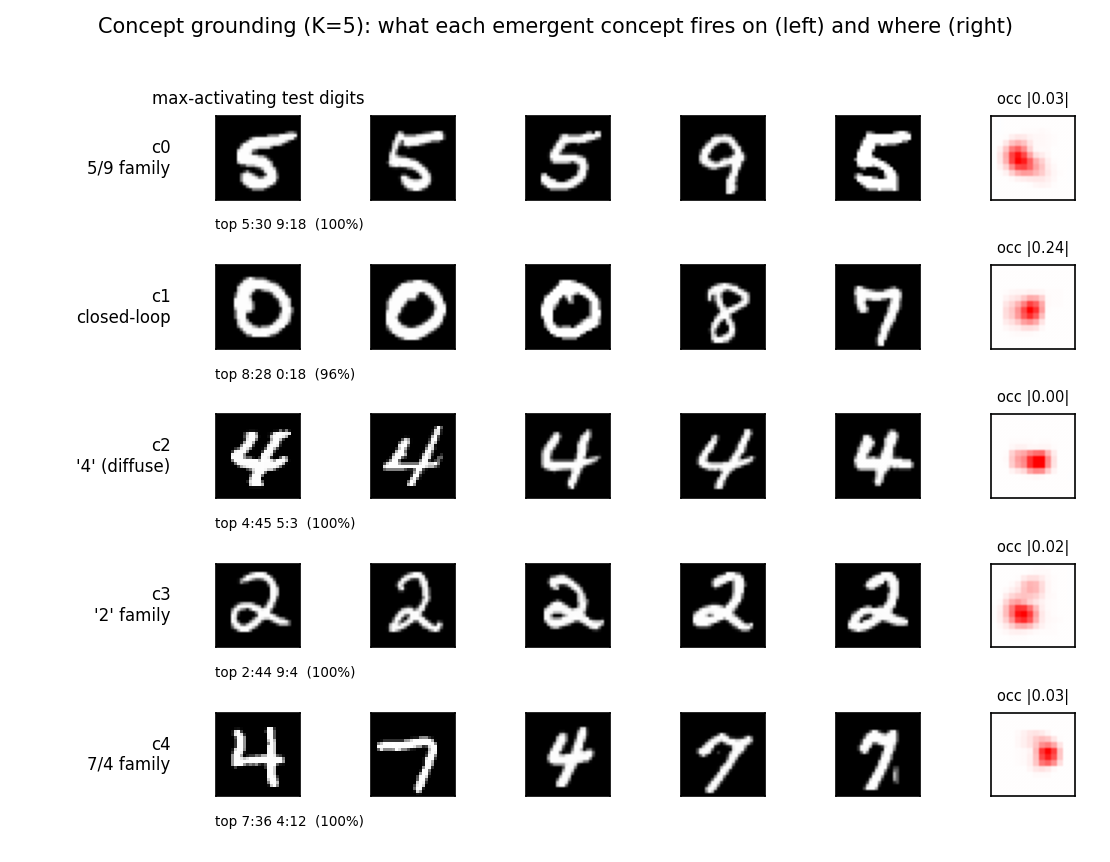
\includegraphics[width=\linewidth]{results/concept_grounding_k5.png}
\caption{Concept grounding for the $K=5$ MNIST OBM. Each row is one emergent
concept: (left) its five maximally activating test digits, (right) its average
occlusion saliency map (red = removing ink there lowers the concept). The
concepts partition digits into visual families; $c_1$ (closed-loop) is the only
one with a strong, localised saliency signature.}
\label{fig:grounding}
\end{figure}

\begin{table}[t]
\centering
\small
\begin{tabular}{clccc}
\toprule
concept & interpretation & top digits & purity & occ.\ peak \\
\midrule
$c_0$ & $5/9$ family        & $5,9$ & $97\%$ & $0.048$ \\
$c_1$ & \textbf{closed loop} & $8,0$ & $92\%$ & $\mathbf{0.320}$ \\
$c_2$ & ``$4$'' (diffuse)   & $4$   & $89\%$ & $0.010$ \\
$c_3$ & ``$2$'' family      & $2$   & $91\%$ & $0.048$ \\
$c_4$ & $7/4$ family        & $7,4$ & $100\%$ & $0.061$ \\
\bottomrule
\end{tabular}
\caption{Concept identity from maximally activating images and occlusion
saliency. \emph{Purity} is the fraction of the top-$48$ activators falling in
the two dominant digit classes; \emph{occ.\ peak} is the maximum average
occlusion sensitivity. Only $c_1$ is a localised abstract primitive.}
\label{tab:concept-identity}
\end{table}

\paragraph{(iii) Faithfulness: do the concepts transfer?}
Finally we test whether each concept encodes a robust visual factor or a
dataset-specific shortcut by applying the frozen MNIST encoder, without any
retraining, to an \emph{external} handwritten-digit corpus (USPS; $2{,}007$
images, resized to $28\times28$ and normalised with the MNIST statistics). For
each concept we report the one-vs-rest AUC of its hypothesised target family on
both corpora and the transfer gap (Table~\ref{tab:concept-transfer}). The
abstract primitive $c_1$ (closed loop) transfers almost perfectly
($0.94\!\rightarrow\!0.92$), and the family detectors $c_0, c_3, c_4$ transfer
well. The diffuse concept $c_2$ degrades the most---its $4$-vs-rest AUC falls
from $0.91$ to $0.73$ and its top-selected digit flips from $4$ to $8$ under the
domain shift---exactly as its near-zero occlusion saliency predicted. Zero-shot
transfer AUC thus doubles as a \emph{label-free faithfulness metric}: it ranks
the abstract, localised concept above the diffuse shortcut, and it does so
without any concept annotation.

\begin{table}[t]
\centering
\small
\begin{tabular}{clccc}
\toprule
concept & target & MNIST AUC & USPS AUC & gap \\
\midrule
$c_1$ & closed loop & $0.94$ & $\mathbf{0.92}$ & $+0.02$ \\
$c_3$ & ``$2$''     & $0.93$ & $0.95$ & $-0.02$ \\
$c_0$ & $5/9$       & $0.91$ & $0.86$ & $+0.04$ \\
$c_4$ & $7/4$       & $0.95$ & $0.86$ & $+0.09$ \\
$c_2$ & ``$4$''     & $0.91$ & $0.73$ & $+0.18$ \\
\bottomrule
\end{tabular}
\caption{Zero-shot concept transfer from MNIST to USPS (one-vs-rest AUC of each
concept for its target family). The abstract concept $c_1$ transfers cleanly;
the diffuse concept $c_2$ degrades most, consistent with its flat occlusion
saliency.}
\label{tab:concept-transfer}
\end{table}

\paragraph{Failure analysis of the weakest concept.}
Because $c_2$ is the concept our diagnostics flag, we examine \emph{how} it
fails under transfer (Fig.~\ref{fig:c2gap}). The MNIST digits that most activate
$c_2$ are all one glyph style---the open-top, angular ``$4$'' that MNIST
over-represents (row A). On USPS, the genuine $4$-signal survives (USPS $4$s
still average $c_2=0.95$), so the AUC drop is \emph{not} a missed-$4$ problem;
it is a false-positive collapse: under USPS's thicker, blurrier strokes $c_2$
saturates on many \emph{non}-$4$ curvy digits---the high-$c_2$ USPS false
positives are dominated by $8$s and $5$s (row C)---destroying the one-vs-rest
ranking. This is precisely the behaviour predicted by $c_2$'s near-zero
occlusion saliency: it responds to a diffuse, global ink statistic rather than a
$4$-shaped region, so a domain shift in stroke statistics makes it fire
indiscriminately. A secondary, smaller effect is genuine coverage: the
lowest-$c_2$ USPS $4$s (row B) are the rounded / closed-top variants that MNIST
under-represents. The transfer-failure visual thus \emph{corroborates} the
occlusion diagnosis with concrete examples rather than restating it.

\begin{figure}[t]
\centering
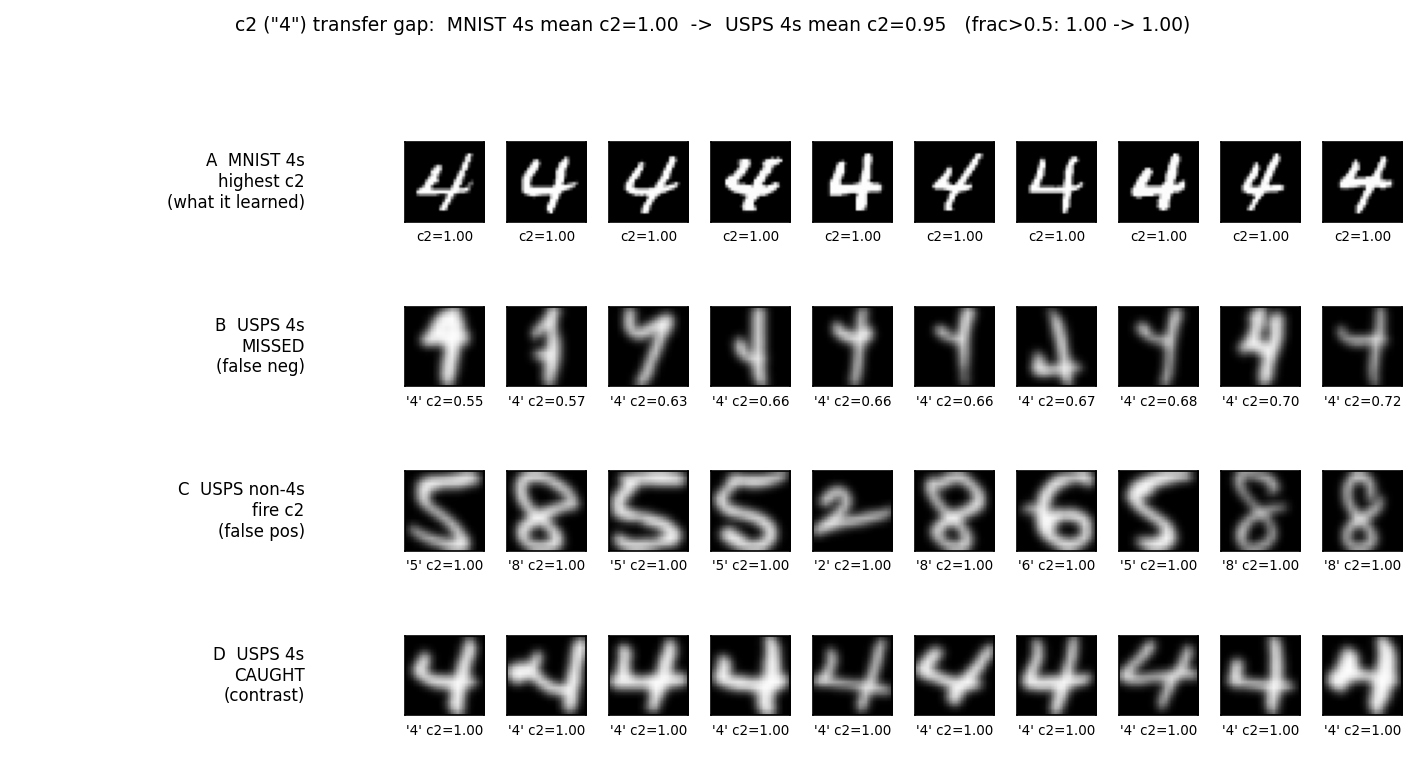
\includegraphics[width=\linewidth]{results/c2_transfer_gap.png}
\caption{Why $c_2$ (``$4$'') fails to transfer. \textbf{A}: MNIST $4$s with
highest $c_2$---all open-top angular. \textbf{B}: USPS $4$s with lowest
$c_2$---rounded / closed-top variants (mild coverage gap). \textbf{C}: USPS
\emph{non}-$4$s that fire $c_2$ (false positives, dominated by $8$/$5$).
\textbf{D}: USPS $4$s that do transfer, matching the MNIST style. The failure is
a false-positive collapse driven by a diffuse, non-localised cue.}
\label{fig:c2gap}
\end{figure}

\paragraph{Concept activation is not concept use.}
A subtle but important consequence is that the concept a digit maximally
\emph{activates} need not be the concept its logic tree \emph{uses}. The
pruned rule for digit $4$ is
\[
\mathcal{A}_{1.08}\!\big[\,\mathcal{A}_{1.40}[c_{1}{:}0.02,\ c_{0}{:}0.98]{:}0.38,\
c_{4}{:}0.62\,\big],
\]
which relies on $c_0$ (junction) and $c_4$ (edge) and does \emph{not} reference
$c_2$ at all---even though $c_2$ is the concept $4$s most activate. The reason is
that maximal activation measures the marginal $P(c_i\!\uparrow\mid y{=}4)$,
whereas the tree selects for \emph{discriminative separation} of $4$ from the
other nine classes. Ranking the concepts by their $4$-vs-rest AUC
(Table~\ref{tab:digit4-use}) shows why: $c_2$ fires at $1.00$ on $4$s but also
averages $0.76$ on non-$4$s (margin $0.24$), whereas $c_4$ fires equally hard on
$4$s yet sits at $0.45$ elsewhere (margin $0.55$) and is in fact the single most
discriminative concept for $4$. The tree therefore picks the two cleanest,
localised separators ($c_4$ edge and $c_0$ junction, both firing on the crossing
of a $4$) and discards the diffuse, high-baseline $c_2$ as redundant. Notably,
the transparent logic head reaches the \emph{same} verdict as our occlusion and
transfer diagnostics---it declines to rely on $c_2$ for the very digit $c_2$
fires on---so the OBM head lets us observe the model auditing and routing around
its own unreliable concept.

\begin{table}[t]
\centering
\small
\begin{tabular}{clccc}
\toprule
concept & role in $4$-tree & $4$-vs-rest AUC & mean on $4$ & mean off $4$ \\
\midrule
$c_4$ & used (edge)      & $\mathbf{0.933}$ & $1.00$ & $0.45$ \\
$c_2$ & \emph{not used}  & $0.909$ & $1.00$ & $0.76$ \\
$c_0$ & used (junction)  & $0.809$ & $0.99$ & $0.63$ \\
$c_3$ & not used         & $0.175$ & $0.37$ & $0.62$ \\
$c_1$ & used (negated)   & $0.070$ & $0.01$ & $0.51$ \\
\bottomrule
\end{tabular}
\caption{Per-concept discrimination for digit $4$. The most-activated concept
($c_2$) is not the most-discriminative: its high off-target baseline ($0.76$)
gives it a smaller margin than $c_4$, which the tree uses instead. Concept
activation $\neq$ concept use.}
\label{tab:digit4-use}
\end{table}

\paragraph{Summary.}
Taken together, the three diagnostics support a precise and honest reading of
what task-only supervision produces. The emergent code is neither a random
scramble nor a rediscovery of pen strokes: it is a near-orthogonal
(Table~\ref{tab:concept-distinctness}) \emph{partition of the label space into
visual families} (Table~\ref{tab:concept-identity}), augmented by one genuinely
abstract, transferable primitive---the closed loop---where the data support it
(Table~\ref{tab:concept-transfer}). The same procedure also flags its own weak
concept ($c_2$), and the transparent logic head is seen to route around that
concept for the very digit it fires on (Table~\ref{tab:digit4-use}), giving the
interpretation a built-in faithfulness check rather than a post-hoc narrative.

\subsection{Transferring the Reasoning, not just the Concepts}
\label{sec:tree-transfer}

The diagnostics above transfer individual concepts. We now transfer the
\emph{entire} learned classifier---encoder $\rightarrow$ $K$ concepts
$\rightarrow$ ten graded-logic digit trees $\rightarrow$ $\arg\max$---to USPS
with no retraining. Accuracy falls from $99.6\%$ (MNIST) to $62.5\%$
(USPS)---well above the $10\%$ chance floor, so the symbolic reasoning does
carry across domains, but the per-digit breakdown reveals a sharp, structured
failure rather than uniform degradation (Table~\ref{tab:tree-transfer}). Almost
every error is the same mistake: the model predicts \emph{8}. True $8$s are only
$8.3\%$ of USPS, yet the model labels $42\%$ of the corpus as $8$ (precision
$19.7\%$); the apparent ``$100\%$ recall'' on $8$ is an attractor sink, not
robustness. Crucially, the other trees keep \emph{high precision} (e.g.\ digit
$4$: recall $48\%$ but precision $91\%$)---when a non-$8$ tree fires it is
usually correct; it simply loses the $\arg\max$ competition to the over-firing
$8$-tree.

\begin{table}[t]
\centering
\small
\begin{tabular}{crrr}
\toprule
digit & USPS recall & USPS prec. & pred.\ share \\
\midrule
$0$ & $92.2\%$ & $97.4\%$ & $16.9\%$ \\
$1$ & $86.4\%$ & $99.6\%$ & $11.4\%$ \\
$7$ & $70.1\%$ & $80.5\%$ & $6.4\%$ \\
$6$ & $61.8\%$ & $94.6\%$ & $5.5\%$ \\
$4$ & $48.0\%$ & $91.4\%$ & $5.2\%$ \\
$5$ & $25.0\%$ & $87.0\%$ & $2.3\%$ \\
$9$ & $\phantom{0}4.5\%$ & $57.1\%$ & $0.7\%$ \\
$8$ & $100.0\%$ & $\mathbf{19.7\%}$ & $\mathbf{42.0\%}$ \\
\bottomrule
\end{tabular}
\caption{Whole-model zero-shot transfer to USPS ($62.5\%$ overall). The errors
are not uniform: the $8$-tree becomes an attractor (predicted for $42\%$ of
images at $19.7\%$ precision) while other trees keep high precision but lose
recall to it. (Digits $2,3$ omitted for space; both behave like $4$.)}
\label{tab:tree-transfer}
\end{table}

\paragraph{Diagnosis via the symbolic structure.}
Because the head is transparent, the failure is mechanistically explainable. The
$8$-tree is $\mathcal{A}[\mathcal{A}[c_2,c_0],c_1]$---closed loop ($c_1$)
\emph{and} junction ($c_0$)---the digit demanding the largest \emph{conjunction}
of concepts to be simultaneously high. Under the domain shift, USPS's thicker,
blurrier strokes shift the concept marginals: the loop concept $c_1$ inflates by
$+0.28$ (mean $0.47\!\rightarrow\!0.75$) and $c_2$ by $+0.08$, while the edge
concept $c_4$ deflates by $-0.23$. Inflating exactly the concepts the $8$-tree
requires makes its conjunction fire for almost any digit, and the
highest-conjunction tree therefore wins the $\arg\max$ competition. A black-box
head would report only ``$62.5\%$, many errors''; the symbolic head names the
culprit (the $8$-tree), the cause (concept-marginal inflation), and the victims
(high-concept-count digits such as $9=$ loop$+$tail).

\paragraph{An unsupervised, targeted fix.}
The diagnosis predicts a remedy that needs no target labels: realign the concept
marginals before the trees. We quantile-match each USPS concept distribution
onto the MNIST reference distribution (source statistics only, concepts remain
in $[0,1]$, per-image concept ranking preserved) and re-run the unchanged trees.
This lifts USPS accuracy from $62.5\%$ to $\mathbf{74.0\%}$ ($+11.5$ points) and
dissolves the attractor: the $8$ prediction share drops from $42\%$ to $17.5\%$
and its precision more than doubles ($19.7\%\!\rightarrow\!46.4\%$). The victim
digits recover in proportion to how badly the attractor had captured them---most
strikingly digit $9$ ($4.5\%\!\rightarrow\!53.1\%$ recall), digit $3$
($46\%\!\rightarrow\!86\%$) and digit $4$ ($48\%\!\rightarrow\!80\%$)
(Table~\ref{tab:tree-calib}). That a purely distributional, label-free
recalibration removes the failure confirms concept-marginal inflation---not the
logic---as the mechanism, and illustrates a general advantage of the OBM: the
transparent head turns a domain-shift failure into a \emph{localised, testable}
hypothesis and a targeted fix, rather than an opaque accuracy drop.

\begin{table}[t]
\centering
\small
\begin{tabular}{lrrr}
\toprule
 & raw & calibrated & $\Delta$ \\
\midrule
USPS accuracy       & $62.5\%$ & $\mathbf{74.0\%}$ & $+11.5$ \\
$8$ prediction share & $42.0\%$ & $17.5\%$ & $-24.5$ \\
$8$ precision        & $19.7\%$ & $46.4\%$ & $+26.7$ \\
\midrule
digit $9$ recall     & $\phantom{0}4.5\%$ & $53.1\%$ & $+48.6$ \\
digit $3$ recall     & $46.4\%$ & $86.1\%$ & $+39.7$ \\
digit $4$ recall     & $48.0\%$ & $80.0\%$ & $+32.0$ \\
\bottomrule
\end{tabular}
\caption{Unsupervised per-concept quantile calibration (MNIST reference,
no USPS labels) dissolves the $8$-attractor and recovers $+11.5$ points,
confirming concept-marginal inflation as the mechanism.}
\label{tab:tree-calib}
\end{table}

\subsection{Debuggability: Diagnosing and Repairing an Overconfident Failure}
\label{sec:debuggability}

OCBM's goal is to let machines and autonomous agents reason in a human-aligned
manner. Because the graded-logic trees are fully transparent, we can inspect the
reasoning process, identify potential weak points, and apply fixes \emph{before}
a failure occurs. Reading the rules in Table~\ref{tab:digit-rules}, we can
anticipate two such weak points. Dense noise saturates every concept, which
should drive the highest-conjunction digit detector to misfire; an empty image
drives every concept low, which should make a detector that relies heavily on
negation misfire. We validated both predictions by constructing the
corresponding attacks---one high-density-noise image and one blank image---and
the outcome was exactly as anticipated: the noise is classified as an
\textbf{$8$} (the strongest conjunction, roundness~$\wedge$~junction) and the
blank as a \textbf{$1$} (recognized largely by the absence of loops and bars),
each at essentially $100\%$ confidence.

This is \emph{not} an OCBM-specific vulnerability: the pathology resides in the
\emph{encoder}, which maps degenerate inputs onto in-distribution concept vectors
before any head sees them. Replacing the graded-logic head with an MLP or a
linear head on the \emph{same task-only bottleneck} (no concept supervision)
leaves the same attacks equally effective. What
those opaque heads do not provide is insight into the failure mechanism---which
rule fired, and on which concept pattern. Armed with that diagnosis, which
localises the fault to out-of-distribution inputs rather than to the logic, we
apply a simple model-agnostic input guard: a percentile box on two cheap image
statistics (the ink fraction and the total variation per unit ink). It rejects
every attack family we tried---blank, uniform noise, Gaussian noise,
salt-and-pepper, and full ink---while keeping $97.9\%$ of real MNIST
(false-reject $2.07\%$) and leaving accuracy on accepted digits unchanged at
$99.6\%$ (Table~\ref{tab:attack-defense}). This study illustrates how OCBM's
transparency lets us analyse and defuse a potential threat before deployment.

\begin{table}[t]
\centering
\small
\begin{tabular}{lr}
\toprule
input family & rejected \\
\midrule
blank (all background)      & $100\%$ \\
uniform noise               & $100\%$ \\
Gaussian noise              & $100\%$ \\
salt-and-pepper             & $100\%$ \\
full ink                    & $100\%$ \\
\midrule
MNIST test (\emph{accepted}) & $97.9\%$ \\
\bottomrule
\end{tabular}
\caption{A two-statistic input sanity check (ink fraction and
total-variation-per-ink, fit on MNIST train; no model internals) rejects every
degenerate-input attack while retaining $97.9\%$ of real MNIST; accuracy on
accepted digits is $99.66\%$. The fix is prescribed by the symbolic diagnosis,
which localises the failure to the input distribution rather than the logic.}
\label{tab:attack-defense}
\end{table}
